% Title of paper
\newcommand{\papertitel}{Title (style: title; Arial 14 pt, bold, left aligned)}

% Speaker
\newcommand{\speaker}{Academic Title, first name, last name, company, country of speaker}

% Co-authors
\newcommand{\coautors}{Academic Title, first name, last name, company, country of co-author\\
	Other co-authors below with the same information, each in a new line\\
	(style: authors; Arial 11 pt, left-aligned)}

% Keywords
\newcommand{\keywords}{Mode-stirred chamber, Reverberation chamber, Statistical distribution, Correlation, Transmission line theory, Immunity test, Electromagnetic compatibility, Directivity, Absorber chamber, Waveguide, DUT model}

% load central settings
\input{Settings}

\section{Main heading 1 (style: heading 1; Arial 11 pt, bold, left aligned)}

Start here with the full paper (style: text body; Arial 11 pt, justification). Graphics, tables etc. can also be inserted here.

Insert references via the \verb|\cite{}| command.

\nocite{source1,source2,source3,source4,source5}

For more information on citing sources, see the IEEE Reference Guide~\cite{ieee:style_manual}.

Finally, reference is made to the example table~\ref{tab:example}.

\begin{table}
	\centering
		\begin{tabular}{@{}p{0.45\textwidth}p{0.45\textwidth}@{}}
			\toprule
			\bfseries Table column head & \bfseries Table column head \\
			\midrule
			Table content & Table content \\
			\midrule
			Table content & Table content \\
			\midrule
			Table content & Table content \\
			\bottomrule
	\end{tabular}
	\caption{Example table (Arial 10 pt, left-aligned, justified if there is a lot of text)}
	\label{tab:example}
\end{table}

An exemplary measurement setup is shown in Figure~\ref{fig:setup}.

\begin{figure}
	\centering
		\begin{tikzpicture}
			% Signal generator
			\node[draw] (sg) {Signal generator};
			% Spectrum analyzer
			\node[draw,right=of sg] (sa) {Spectrum analyzer};
			% Connecting arrow
			\draw[->] (sg) -- (sa);
		\end{tikzpicture}
	\caption{Measurement setup (Subtitle picture, Arial 10 pt, left-aligned, justified if there is a lot of text)}
	\label{fig:setup}
\end{figure}

An exemplary measurement result is shown in Figure~\ref{fig:result}.

\begin{figure}
	\centering
		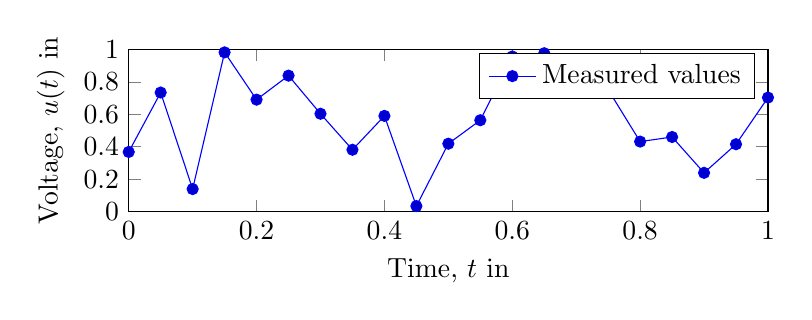
\begin{tikzpicture}
			\begin{axis}[
				xlabel={Time, $t$ in \si{\second}},
				ylabel={Voltage, $u(t)$ in \si{\volt}},
				width=0.8\textwidth,
				height=0.3\textwidth,
				xmin=0,xmax=1,
				ymin=0,ymax=1,
				]
				\addplot+[
					domain=0:1,
					samples=21,
				]{rnd};
				\addlegendentry{Measured values}
			\end{axis}
		\end{tikzpicture}
	\caption{Measurement result (Subtitle picture, Arial 10 pt, left-aligned, justified if there is a lot of text)}
	\label{fig:result}
\end{figure}

%An example tabular listing is shown in table~\ref{tab:example_table}.
%
%\begin{table}
	%\centering
		%\begin{tabular}{@{}p{0.15\textwidth}p{0.15\textwidth}p{0.15\textwidth}p{0.15\textwidth}p{0.15\textwidth}@{}}
			%\toprule
			%Lorem & Ipsum & Dolor & Sit & Amet \\
			%\midrule
			%consectetuer & sed diam & sed diam & sed diam & sed diam \\
			%\midrule
			%adipiscing & sed diam & sed diam & sed diam & sed diam \\
			%\midrule
			%elit & sed diam & sed diam & sed diam & sed diam \\
			%\bottomrule
	%\end{tabular}
	%\caption{Example table (Arial 10 pt, left-aligned, justified if there is a lot of text)}
	%\label{tab:example_table}
%\end{table}

Examples of headings are shown below. Good luck with your writing project!

\subsection{Subtitle 1 (style: heading 2; Arial 11 pt, bold, left aligned)}

Here you can insert intermediate topics (style: text body; Arial 11 pt, justification).

%\blindtext

\subsubsection{Subtitle 2 (style: heading 3; Arial 11 pt, left-aligned)}

%Here you can insert further subthemes (Arial 11 pt, justified).

\paragraph{Subtitle 4 (style: heading 3; Arial 11 pt, left-aligned)}

Text for the next sub-item (style: text body; Arial 11 pt, justification).

\section{Notes on the format templates for the captions}

Captions of the figures should be labeled as shown below:

\begin{figure}
	\caption{Caption (style: caption; Arial 10 pt, left-justified, with a lot of text justified)}
\end{figure}

Tables should be labeled as shown below:

\begin{table}
	\caption{Table caption (style: caption; Arial 10 pt, left-justified, with a lot of text justified)}
\end{table}

% list of references using BibTeX
%\bibliographystyle{plaindin}	% German DIN style
%\bibliographystyle{ieeetran}	% IEEE style
%\bibliography{literature}
% List of references using biblatex
\printbibliography

\end{document}
